\documentclass{frontiersSCNS}
%\documentclass{article}
%\usepackage{biblatex}
%\usepackage{amsmath}
%\usepackage{amssymb}
%\usepackage{times}
\usepackage{hyperref}
%\usepackage{graphicx}
\usepackage{wrapfig}
\usepackage{listings}
%\usepackage[usenames,dvipsnames]{xcolor}
%\usepackage{setspace}
\usepackage{python_syntax}
%\usepackage{bibentry}
\usepackage{todonotes}
\usepackage{url}
\usepackage{lineno}
\usepackage{upquote}
%\usepackage{natbib}
%\usepackage{caption}

%\usepackage{biblatex}
%\DeclareCiteCommand{\wcite}
%    [\mkbibfootnote]
%    {}
%    {\printfield{title}--\printfield{howpublished}}
%    {\addcomma\addspace}
%    {}

\usepackage[english]{babel} 
\def\UrlFont{\em} % Italicize all URLs.  
\lstset{
	basicstyle=\small\ttfamily,
	breaklines=true,
	language=Python,
	}
\let\verbx\lstinline
\newcommand{\bfhead}[1]{\noindent \textbf{#1:}}

\linenumbers
\copyrightyear{}
\pubyear{}

\def\journal{NeuroInformatics}%%% write here for which journal %%%
\def\DOI{}
\def\articleType{Methods}
\def\keyFont{\fontsize{8}{11}\helveticabold }
\def\firstAuthorLast{Sample {et~al.}} %use et al only if is more than 1 author
\def\Authors{Richard C. Gerkin\,$^{1,*}$ and Cyrus Omar\,$^{2}$}
% Affiliations should be keyed to the author's name with superscript numbers and be listed as follows: Laboratory, Institute, Department, Organization, City, State abbreviation (USA, Canada, Australia), and Country (without detailed address information such as city zip codes or street names).
% If one of the authors has a change of address, list the new address below the correspondence details using a superscript symbol and use the same symbol to indicate the author in the author list.
\def\Address{$^{1}$School of Life Sciences, Arizona State University, Tempe, AZ, USA \\
$^{2}$Dept. of Computer Science, Carnegie Mellon University, Pittsburgh, PA, USA  }
% The Corresponding Author should be marked with an asterisk
% Provide the exact contact address (this time including street name and city zip code) and email of the corresponding author
\def\corrAuthor{Rick Gerkin}
\def\corrAddress{ISTB-1 476}
\def\corrEmail{rgerkin@asu.edu}

% \color{FrontiersColor} Is the color used in the Journal name, in the title, and the names of the sections.

\begin{document}

\onecolumn
\firstpage{1}

\title[Running Title]{Collaboratively Testing the Validity of Neuroscientific Models}
\author[\firstAuthorLast ]{\Authors}
\address{}
\correspondance{}
\extraAuth{}% If there are more than 1 corresponding author, comment this line and uncomment the next one.
%\extraAuth{corresponding Author2 \\ Laboratory X2, Institute X2, Department X2, Organization X2, Street X2, City X2 , State XX2 (only USA, Canada and Australia), Zip Code2, X2 Country X2, email2@uni2.edu}
\topic{Python in Neuroscience II}% If your article is part of a Research Topic, please indicate here which.

\maketitle

\begin{abstract}
Rigorously validating a quantitative scientific model requires comparing its predictions against an unbiased selection of experimental observations according to sound statistical criteria. 
Developing new models thus requires a comprehensive and contemporary understanding of competing models, relevant data and statistical best practices. 
Today, developing such an understanding requires an encyclopedic knowledge of the literature. 
Unfortunately, in rapidly-growing fields like neuroscience, this is becoming increasingly untenable, even for the most conscientious scientists. 
For new scientists, this can be a significant barrier to entry.

%However, today's model validation process is based on one-time peer review of a scientific publication. , and thus remains an informal and incomplete process, particularly in fields like neuroscience where the number of competing models and the volume of relevant data is growing rapidly.   
%This makes it difficult to determine community-accepted validation criteria, compare competing models,  determine the state-of-the-art given the latest experimental data, and to precisely identify open modeling problems.

Software engineers seeking to verify, validate and contribute to a complex software project rely not only on volumes of human documentation, but on suites of simple executable tests, called ``unit tests''. 
Drawing inspiration from this practice, we have developed \textit{SciUnit}, an easy-to-use framework for developing ``model validation tests'' -- 
executable functions, here written in Python. 
These tests generate and statistically validate predictions from a specified class of scientific models against one relevant empirical observation to produce a score indicating agreement between the model and the data. 
Suites of such validation tests, collaboratively developed by a scientific community in common repositories, produce up-to-date statistical summaries of the state of the field. In this paper, we aim to detail this test-driven workflow and introduce it to the neuroscience community. 
As an initial example, we describe \textit{NeuronUnit}, a library that builds upon \textit{SciUnit} and integrates with several existing neuroinformatics resources to support validating single-neuron models using data gathered by neurophysiologists. 

\tiny
 \keyFont{ \section{Keywords:} Neuroinformatics Simulation Electrophysiology Software Modeling Validation } %All article types: you may provide up to 8 keywords; at least 5 are mandatory.
\end{abstract}

% Section 1.
\section{Introduction}
\label{sec:introduction}
Neuroscientists construct quantitative models to coherently explain experimental observations of neurons, circuits, brain regions and behavior. 
A model can be characterized by its \textit{scope}: the set of observable quantities that it can generate predictions about, and by its \textit{validity}: the extent to which its predictions agree with available experimental  observations of those quantities.

Today, scientists contribute a new model to the research community by submitting a paper containing a description of the model's structure and scope along with text and figures that demonstrate its validity and argue for its novelty.  
The scientists tasked with reviewing the paper are  responsible for evaluating these claims, discovering competing models and relevant data the paper did not adequately consider, and ensuring that goodness-of-fit was measured in a statistically sound manner, drawing on their knowledge of prior literature. 
Once a modeling paper is published, it is frozen and cited as-is in perpetuity. 

Because publications are the sole vehicle for knowledge about model scope and validity, scientists must rely on an encyclopedic knowledge of the literature to answer \emph{summary questions} like the following:
\begin{itemize}
\item Which models are capable of predicting the quantities I am interested in?
\item What are the best practices for evaluating the goodness-of-fit between these models and  data?
\item How well do these models perform, as judged by these metrics, given currently available data?
\item What other quantities can and can't these models predict?
\item What observations have not yet been adequately explained by any available model?
\end{itemize}

In some fields, like neuroscience, where the number of relevant publications being generated every year is growing rapidly \citep{jinha_article_2010}, these questions can be difficult for even conscientious senior scientists to answer comprehensively. 
For new scientists, this represents a serious barrier to entry. 

%This suggests that tools that help researchers answer questions like these could help readers and reviewers develop a more comprehensive understanding of the state-of-the-art and improve the quality of the research being published as a result: to renewed calls for tools that help researchers . 


%These questions are particularly relevant for young scientists and  scientists aiming to enter a new research area to answer.

%understanding of the state-of-the-art from publications containing only a few pieces of data, and then only that data available at the time of publication. 

%These demonstrations also quickly go out of date. Finally, there is no easy way to summarize and compare the claims being made in modeling papers in order to synthesize an understanding of a research area as a whole. 
%A strength of publications are their focused descriptions of new data and models. 
%A weakness, however, is that evaluating the scope and validity of models against known data is intractable using a body of publications alone.

Professional software developers face similar issues \citep{omar_sciunit_2013}. 
They must understand the scope of each component of a complex software project and verify that each component achieves desired input/output behavior. 
But software developers do not verify components by simply documenting a few interesting inputs and corresponding outputs and then presenting them to other developers for one-time review leading to an archived document. 
Rather, they typically follow a \emph{test-driven development} methodology by creating a suite of executable \emph{unit tests} that serve to specify each component's scope and verify its implementation on an ongoing basis as it is being developed and modified \citep{beck2003}. 
Each test individually checks that a small portion of the program meets a single correctness criterion. 
For example, a unit test might verify that one function within the program correctly handles malformed inputs. 
Collectively, the test results serve as a summary of the project as it progresses through its development cycle. 
Developers can determine which features are unimplemented or buggy by examining the set of failed tests, and progress can be measured in terms of how many tests the program passes over time. 
This methodology is widely adopted in practice \citep{beck2003}.

%publications would be analagous to user manuals, rather than rigorous justifications that a program meets a specific specification. Unit tests serve this purpose for software, so we argue that the validation of neuroscience models by means of executable tests would be useful to scientists as a supplement the publication system.

Test-driven methodologies have started to see success in neuroscience as well, in the form of \emph{modeling competitions}. 
During these competitions, competitors develop and parameterize models based on publicly-available training data and submit them to a central server. 
There, submitted models are provided hidden testing data which they must use to produce predictions. 
These predictions are validated using publicly available criteria to produce summaries of the relative merits of different models, just as a test suite summarizes the state of a software project. 
Such competitions continue to drive important advances and improve scientists' understanding of their fields. 
For example, the quantitative single neuron modeling competition (QSNMC) \citep{jolivet_quantitative_2008} investigated the complexity-accuracy tradeoff among reduced models of excitable membranes; 
the ``Hopfield'' challenge \citep{hopfield_what_2000} tested techniques for generating neuronal network form given its function; 
the Neural Prediction Challenge sought the best stimulus reconstructions, given neuronal activity (\url{http://neuralprediction.berkeley.edu}); the Diadem challenge is advancing the art of neurite reconstruction (\url{http://www.diademchallenge.org}); and 
examples from other areas of biomedical research abound (e.g. \url{http://www.the-dream-project.org}).
% \begin{figure}%{r}{0.6\textwidth}
% %\vspace{-38px}
% 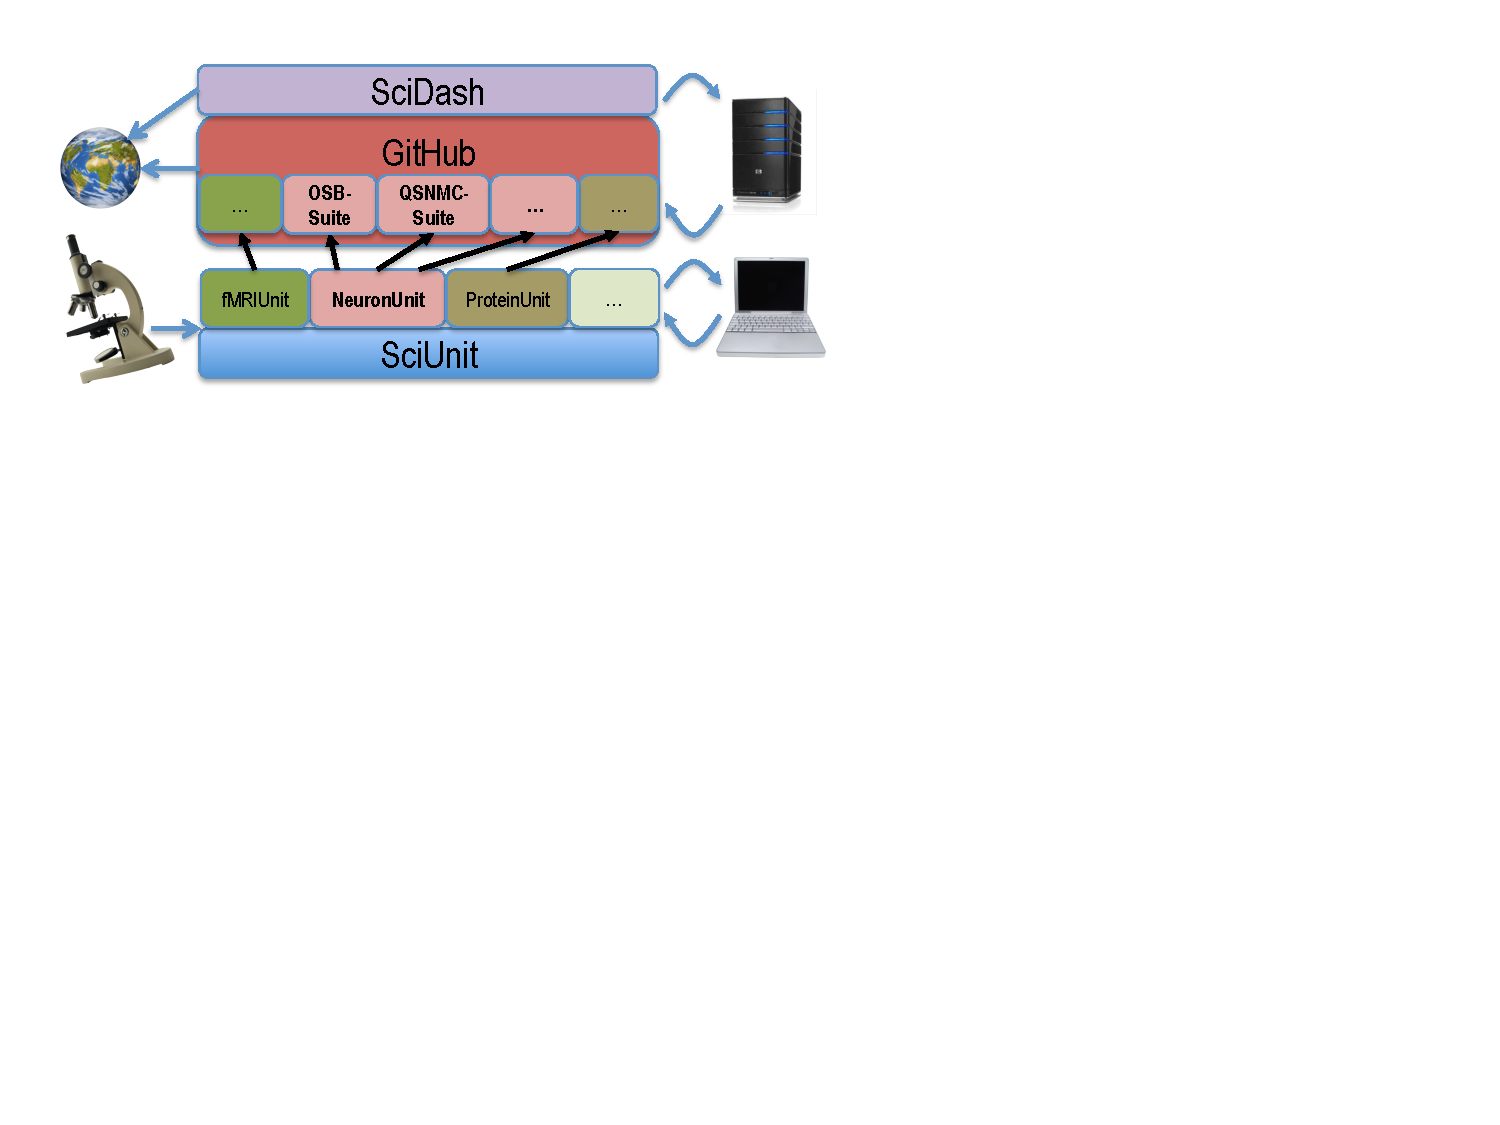
\includegraphics[scale=0.75]{sciunit_overview.pdf}
% \caption{Proposal overview. 
% \small{i) The \textit{SciUnit} framework can generate discipline-specific libraries for tests generation and model interfacing.  
% \textit{NeuronUnit} is proposed and described here.  Experimental data guides test development; model generation informs and is informed by these \textit{SciUnit} libraries.  
% Test suites for OSB and QSNMC (described in the text) are being built. 
% %\vspace{-10px}
% \label{fig:sciunit_overview}
% \end{figure}
% \leavevmode
% \vspace{-0px}
\begin{figure}
\vspace{-45px}
\centering
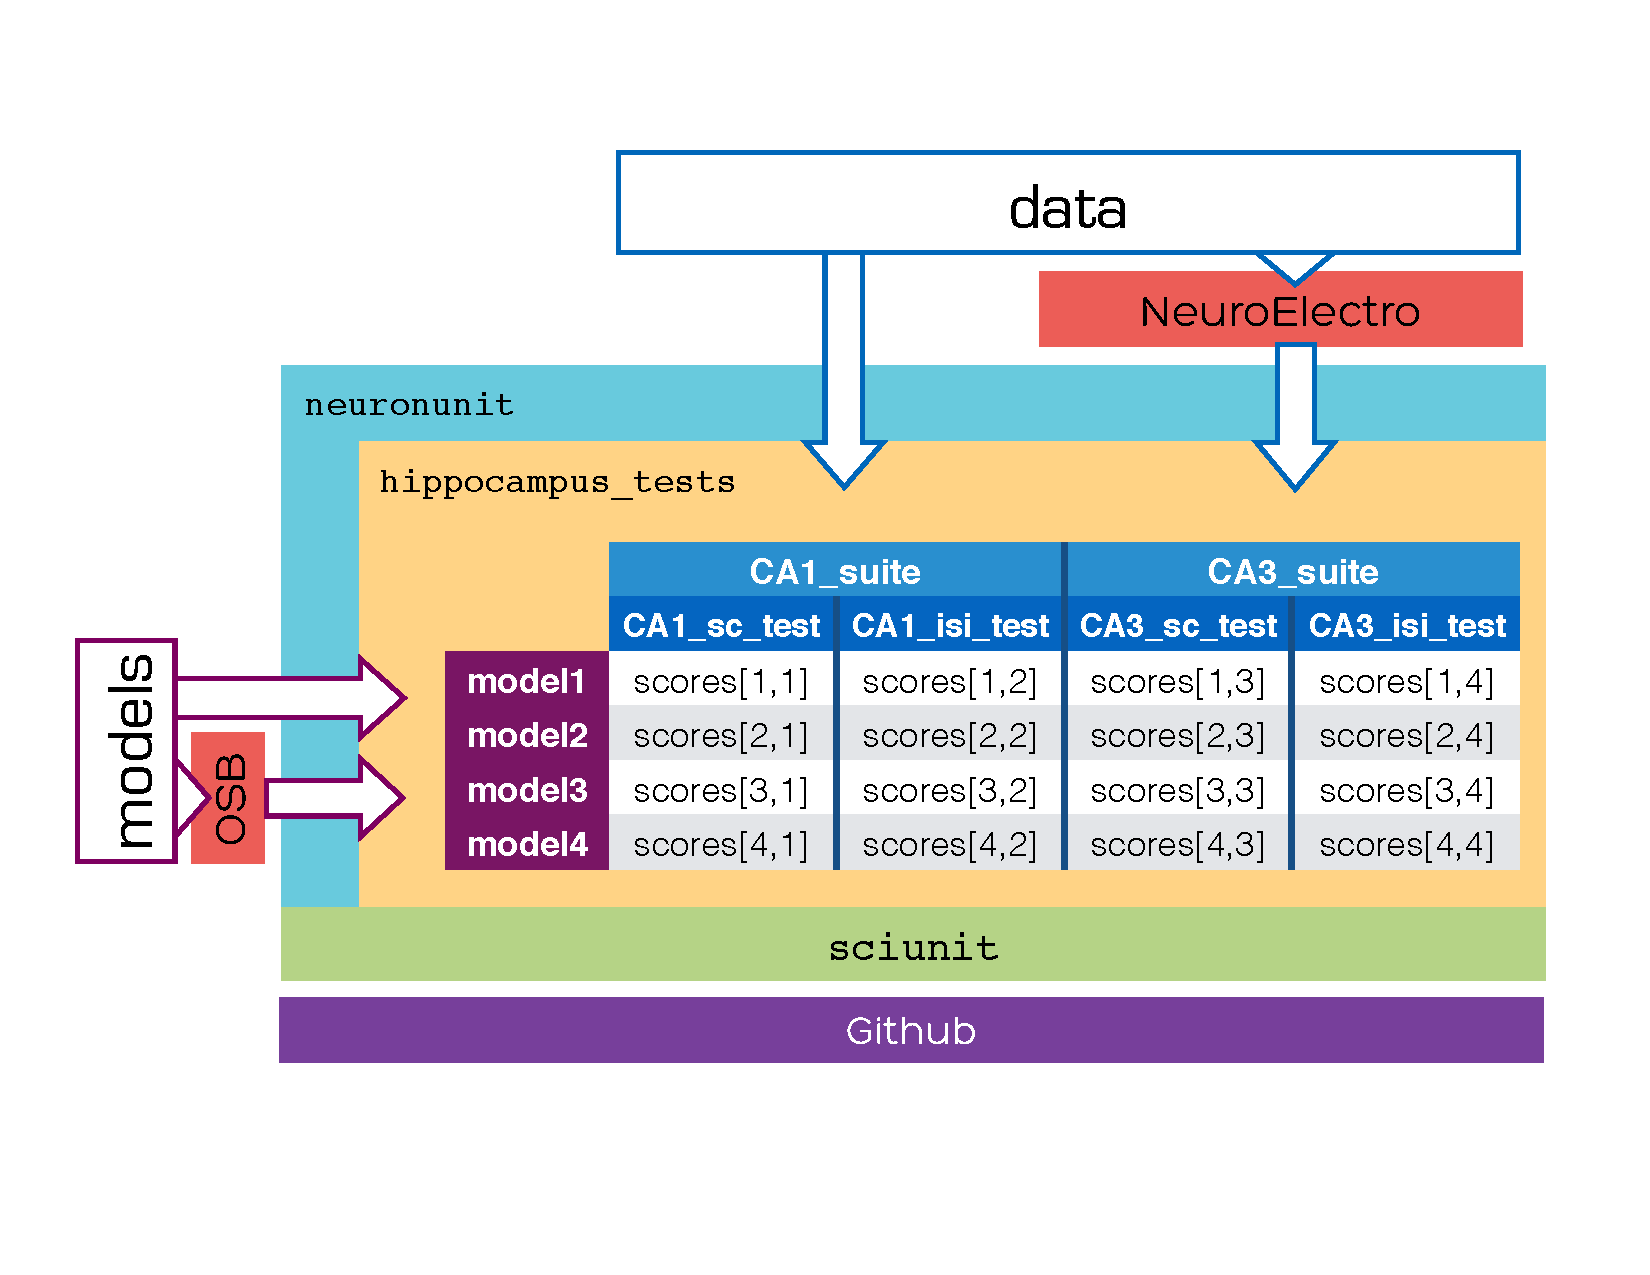
\includegraphics[scale=0.6]{diagram1.pdf}
\vspace{-65px}
\caption{Paper overview. NeuronUnit is set of neurophysiology-specific testing tools built upon the domain-agnostic SciUnit framework. 
Scientists interested in testing neurophysiological models of particular systems, like the hippocampus, against relevant experimental data can construct test suites in a repository called \textit{hippocampus\_tests}. 
Models and data can be added directly or imported, via NeuronUnit, from model repositories like Open Source Brain (OSB) and data repositories like NeuroElectro. 
Testing tools and test repositories are developed collaboratively using Github.}  
\label{fig:sciunit_overview}\vspace{-10px}
\end{figure}
\leavevmode


Each of these examples has leveraged \emph{ad hoc} infrastructure to support model validation. 
While the specific criteria used to evaluate models can vary widely between modeling domains, the underlying methodology is common and could be implemented once. 
Recognizing this, and inspired by unit testing practices, we have developed a discipline-agnostic framework for developing \emph{model validation test suites} called \textit{SciUnit} \citep{omar_sciunit_2013} (available from \url{http://sciunit.scidash.org}). 
In this paper, we will begin by detailing \textit{SciUnit}, focusing on examples from single-neuron physiology (Sec. \ref{sec:sciunit}). 

\textit{SciUnit} contains validation logic common across scientific disciplines.
But a particular discipline, such as neurophysiology, might have more specialized logic associated with it that can be shared amongst its sub-disciplines (e.g. hippocampal neurophysiology). 
We anticipate a collaborative workflow where this common logic is developed in common repositories on a social coding service, here \textit{GitHub}. 
For neurophysiology, we have developed such a repository, called \textit{NeuronUnit}. 
This repository contains common testing logic as well as bridges to existing informatics infrastructure to make it easy to import existing data and models. 
In particular, we will show how models described using \text{NeuroML} and provided freely by the \textit{Open Source Brain Project} (OSB, \cite{gleeson_open_2012}, \url{http://www.opensourcebrain.org}) can be tested in a fully automated fashion using published data curated by the \textit{NeuroElectro Project} (NeuroElectro, \cite{tripathy_neuroelectro:_2012}, \url{http://neuroelectro.org}), leveraging facilities from the \textit{NeuroTools} library (\url{http://neuralensemble.org/NeuroTools}) to extract features from model outputs (Sec. \ref{sec:neuronunit}). 
Scientists in particular sub-disciplines, like hippocampal neurophysiologists, can use this common logic to select relevant models and tests, forming focused test suites in common repositories. 
The end result of this workflow is a table like the one shown in Figure \ref{fig:sciunit_overview}, where submitted models can be compared based on the scores they achieve on different selected tests. 
These tables serve as a summary of the status of a modeling community, just as the results from a suite of unit tests serve as a summary of the status of a software project, and help scientists answer the questions mentioned earlier in this section more easily and accurately.

% Section 2.
\section{Validation Testing with \textit{SciUnit}}\label{sec:sciunit}
\subsection{Example: The Quantitative Single Neuron Modeling Competition}\label{sec:example}
\begin{figure}
\small
\begin{python}
class SpikeCountTest(sciunit.Test):
  """Tests spike counts produced in response to several current stimuli against observed means and standard deviations. 

  goodness of fit metric: Computes p-values based on a chi-squared test statistic, and pools them using Fisher's method.
  parameters:
    inputs: list of numpy arrays containing input currents (nA)
    means, stds: lists of observed means and standard deviations, one per input
  """
  def __init__(self, inputs, means, stds):
    self.inputs, self.means, self.stds = inputs, means, stds
	
  required_capabilities = [SpikeCountFromCurrent]
	
  def _judge(self, model):
    inputs, means, stds = self.inputs, self.means, self.stds
    n = len(inputs)
    counts = numpy.empty((n,))
    for i in xrange(n):
      counts[i] = model.spike_count_from_current(inputs[i])
    chisquared = sum((counts-means)**2 / means) # An array of chi-squared values.  
    p = scipy.stats.chi2.cdf(chisquared,n-1) # An array of p-values.  
    pooled_p = sciunit.utils.fisherp(p_array) # A pooled p-value.  
    return sciunit.PValue(pooled_p, related_data={
      "inputs": inputs, "counts": counts, "obs_means": means, "obs_stds": stds
    })
\end{python}
\vspace{-15px}
\caption{\texttt{[neuronunit.SpikeCountTest]} An example single neuron spike count test class implemented using \textit{SciUnit}. Because this implementation contains logic common to many different systems, \textit{NeuronUnit} was developed to provide a simpler means to deliver it (see Sec. \ref{sec:neuronunit}).}
\label{fig:rate_test}
\vspace{-10px}
\end{figure}

%Simple executable \emph{validation tests} that compute agreement between a model prediction and an experimental observation.  
We begin by building an example \textit{SciUnit} test suite that could be used in neurophysiology. 
Suppose we have collected data from an experiment where current stimuli (measured in pA) are delivered to neurons of a particular subtype, while the somatic membrane potential of each stimulated cell (in mV) is recorded and stored.  
A model claiming to capture this neuron type's membrane potential dynamics must be able to accurately predict a variety of features observed in these data.

One simple validation test would ask candidate models to predict the number of action potentials (a.k.a. spikes) generated in response to a stimulus (e.g. white noise), and compare these \emph{spike count} predictions to the distribution observed in repeated experimental trials using the same stimulus. 
For data of this type, goodness-of-fit can be measured by first calculating a p-value from a chi-squared statistic for each prediction and then combining these p-values using Fisher's method \citep{fisher_statistical_1925}. 

Alongside this \emph{spike count test}, we might also specify a number of other tests capturing different features of the data  to produce a more comprehensive suite. 
For data of this sort, the QSNMC defined 17 other validation criteria in addition to one based on the overall spike count, capturing features like spike latencies (SL), mean subthreshold voltage (SV), interspike intervals (ISI) and interspike minima (ISM) that can be extracted from the data \citep{jolivet_quantitative_2008}. 
They then defined a combined metric favoring models that broadly succeeded at meeting these criteria, to produce an overall ranking. 
Such combined criteria are simply validation tests that invoke other tests to produce a result.
 
%In many cases, models require no modifications to take the new tests because the same type of model output is being requested.
\subsection{Implementing a Validation Test in \textit{SciUnit}}
Fig. \ref{fig:rate_test} shows how a scientist can implement spike count tests such as the one described above using \textit{SciUnit}. 
A \textit{SciUnit} validation test is an {instance} (i.e. an object) of a Python class implementing the \verbx{sciunit.Test} interface (cf. line 1). 
Here, we show a class \verbx{SpikeCountTest} taking three \emph{parameters} in its constructor (constructors are named \verbx{__init__} in Python, lines 9-10). 
The meaning of each parameter along with a description of the goodness-of-fit metric used by the test is documented on lines 4-7. 
%For convenience, we also make use of functions provided by the popular NumPy\cite{numpy_url} and SciPy\cite{scipy_url} libraries, although these are not required by \textit{SciUnit}.  
To create a \emph{particular} spike count test, we instantiate this class with particular experimental observations. 
For example, given observations from CA1 cells (not shown), we can instantiate a test as follows:
\begin{ipy}
  In [0]: CA1_sc_test = SpikeCountTest(CA1_inputs, CA1_means, CA1_stds)
\end{ipy}
We emphasize the crucial distinction between the \textit{class} \verbx{SpikeCountTest}, which defines a \emph{parameterized family} of validation tests, and the particular \textit{instance} \verbx{CA1_sc_test}, which is an individual validation test because the necessary parameters, derived from data, have been provided. 
As we will describe below, we expect communities to build repositories of such families capturing the criteria used in their subfields of neuroscience so that test generation for a particular system of interest will often require simply instantiating a previously-developed family with particular experimental parameters and data. 
For single-neuron test families like \verbx{SpikeCountTest}, we have developed such a library, called \textit{NeuronUnit} (\url{http://github.com/scidash/neuronunit}) (Sec. \ref{sec:neuronunit}). 
Particular tests, like \verbx{CA1_sc_test}, will be derived from these families in suite repositories (e.g. \verbx{HippocampusTests}, as shown in Figure \ref{fig:sciunit_overview}).

Classes that implement the \verbx{sciunit.Test} interface must contain a \verbx{_judge} method that receives a candidate \emph{model} as input and produces a \textit{score} as output. 
To specify the interface between the test and the model, the test author provides a list of \emph{capabilities} in the \verbx{required_capabilities} attribute, seen on line 12 of Fig. \ref{fig:rate_test}. 
Capabilities are simply collections of methods that a test needs a model to implement so that it can provide inputs and generate relevant predictions, and are analogous to \emph{interfaces} in e.g. Java (\url{http://docs.oracle.com/javase/tutorial/java/concepts/interface.html}). 
In Python, capabilities are written as classes with unimplemented members. 
The capability required by the test in Fig. \ref{fig:rate_test} is shown in Fig. \ref{fig:capability}. 
In \textit{SciUnit}, classes defining capabilities are tagged as such by inheriting from \verbx{sciunit.Capability}. 
The test in Figure \ref{fig:rate_test} uses this capability on line 19 to produce a spike count prediction for each input current. 

The remainder of the \verbx{_judge} method implements the goodness-of-fit metric described above, returning an instance of \verbx{sciunit.PValue}, a subclass of \verbx{sciunit.Score} that is included with \textit{SciUnit}. 
In addition to the $p$-value itself, the returned score object also contains metadata, via the \verbx{related_data} parameter, for scientists who may wish to examine the result in more detail later. 
In this case we save the input currents, the model outputs and the observed means and standard deviations (line 24). 

\begin{figure}
\begin{python}
class SpikeCountFromCurrent(sciunit.Capability):
  def spike_count_from_current(self, input): 
    """Takes a numpy array containing current stimulus (in nA) and
    produces an integer spike count. Can be called multiple times."""
    raise NotImplementedError("Model does not implement capability.")
\end{python}
\vspace{-15px}
\caption{\texttt{[neuronunit.SpikeCountFromCurrent]} An example capability specifying a single required method (used by the test in Figure \ref{fig:rate_test}).}
\label{fig:capability}
\vspace{-10px}
\end{figure}
\begin{figure}
\begin{python}
class TrainSpikeCountFromCurrent(sciunit.Capability):
  def train_with_currents(self, currents, counts):
    """Takes a list of numpy arrays containing current stimulus (in nA) and
    observed spike counts. Model parameters should be adjusted based on this
    training data."""
    raise NotImplementedError("Model does not implement capability.")
\end{python}
\vspace{-15px}
\caption{\texttt{[neuronunit.TrainSpikeCountFromCurrent]} Another capability specifying a training protocol (not used by the test in Figure \ref{fig:rate_test}).}
\label{fig:training}
\vspace{-10px}
\end{figure}

\subsection{Models}
Capabilities are \emph{implemented} by models. 
In \textit{SciUnit}, models are instances of Python classes that inherit from \verbx{sciunit.Model}. 
Like tests, the class itself represents a family of models, parameterized by the arguments of the constructor. 
A particular model is an instance of such a class.

Figure \ref{fig:simple_model} shows how to write a simple {family} of models, \verbx{LinearModel}, that implement the capability in Fig. \ref{fig:capability} as well as another capability shown in Fig. \ref{fig:training}, which we will discuss below. 
Models in this family generate a spike count by applying a linear transformation to the mean of the provided input current. 
The family is parameterized by the scale factor and the offset of the transformation, both scalars. 
To create a \emph{particular} linear model, a modeler provides parameter values, just as with test families:
\begin{ipy}
  In [1]: CA1_linear_model_heuristic = LinearModel(3.0, 1.0)
\end{ipy}
Here, the parameters to the model were picked by the modeler heuristically, or based on externally-available knowledge. 
An alternative test design would add a training phase where these parameters were fit to data using the capability shown in Fig. \ref{fig:training}. 
This alternative test could thus only be used for those models for which parameters can be adjusted without human involvement. 
Whether to build a training phase into the test protocol is a choice left to each test development community. 
Fig. \ref{fig:rate_test} does not include a training phase. 
If training data is externally available, models that nevertheless are capable of being automatically trained (like \verb|LinearModel|) can simply be trained explicitly by calling the capability method just like any other Python method:
\begin{ipy}
  In [2]: CA1_linear_model_fit = LinearModel()
  In [3]: CA1_linear_model_fit.train_with_currents(CA1_training_in, CA1_training_out)
\end{ipy}
\begin{figure}
\begin{python}
class LinearModel(sciunit.Model, SpikeCountFromCurrent, 
    TrainSpikeCountFromCurrent):
  def __init__(self, scale=None, offset=None): 
    self.scale, self.offset = scale, offset
    
  def spike_count_from_current(self, input):
    return int(self.scale*numpy.mean(input) + self.offset)

  def train_with_currents(self, currents, counts):
    means = [numpy.mean(c) for c in currents]
    [self.offset, self.scale] = numpy.polyfit(means, counts, deg=1)    
\end{python}
\vspace{-15px}
\caption{\texttt{[neuronunit.LinearModel]} A model that returns a spike count by applying a linear transformation to the mean input current. The parameters can be provided manually or learned from data provided by a test or user (see text).}
\label{fig:simple_model}
\vspace{-10px}
\end{figure}

\subsection{Executing Tests} A test is executed against a model using the \verbx{judge} method:
\begin{ipy}
  In [4]: score = CA1_sc_test.judge(CA1_linear_model_heuristic)
\end{ipy}

\verbx{judge} is a stock \verbx{sciunit.Test} method that proceeds by first checking that the provided model implements all required capabilities. 
It then calls the test's author-implemented \verbx{_judge} method (note leading underscore) to produce a score. 
A reference to the test and model are added to the score for convenience (accessible via the \verbx{test} and \verbx{model} attributes, respectively), before it is returned.

\subsection{Test Suites and Score Matrices}\label{sec:visualization} A collection of tests intended to be run on the same model can be put together to form a test suite.
The following test suite could be used for a simplified version of the QSNMC, as described in Sec. \ref{sec:example}:  
\begin{ipy}
  In [5]: CA1_suite = sciunit.TestSuite([CA1_overall_test, CA1_sc_test, CA1_sl_test, CA1_sv_test, 
              CA1_isi_test, CA1_imi_test])
\end{ipy}
Like a single test, a test suite is capable of judging one or more models. 
The models must possess the union of the capabilities of the tests in a suite to be fully capable of running the suite, though partial results can also be generated. 
When a model cannot take a test because of a missing capability, the \texttt{NotApplicable} score is used (e.g. point processes cannot predict subthreshold voltages). 
The result is a \emph{score matrix}, like the one diagrammed in Fig. \ref{fig:sciunit_overview}.
\begin{ipy}
  In [6]: scores = CA1_suite.judge([ARX_model, AdEx1_model, aSRM_model, PP_model])
\end{ipy}
A simple summary of the scores in a score matrix can be printed to the console or visualized by other tools.  
For example, the score matrix can be visualized as a hyperlinked table inside an IPython notebook \citep{perez_ipython_2007} (Fig. \ref{fig:scidash_matrix}).


\begin{figure}%[18]{r}{1\textwidth}
\centering
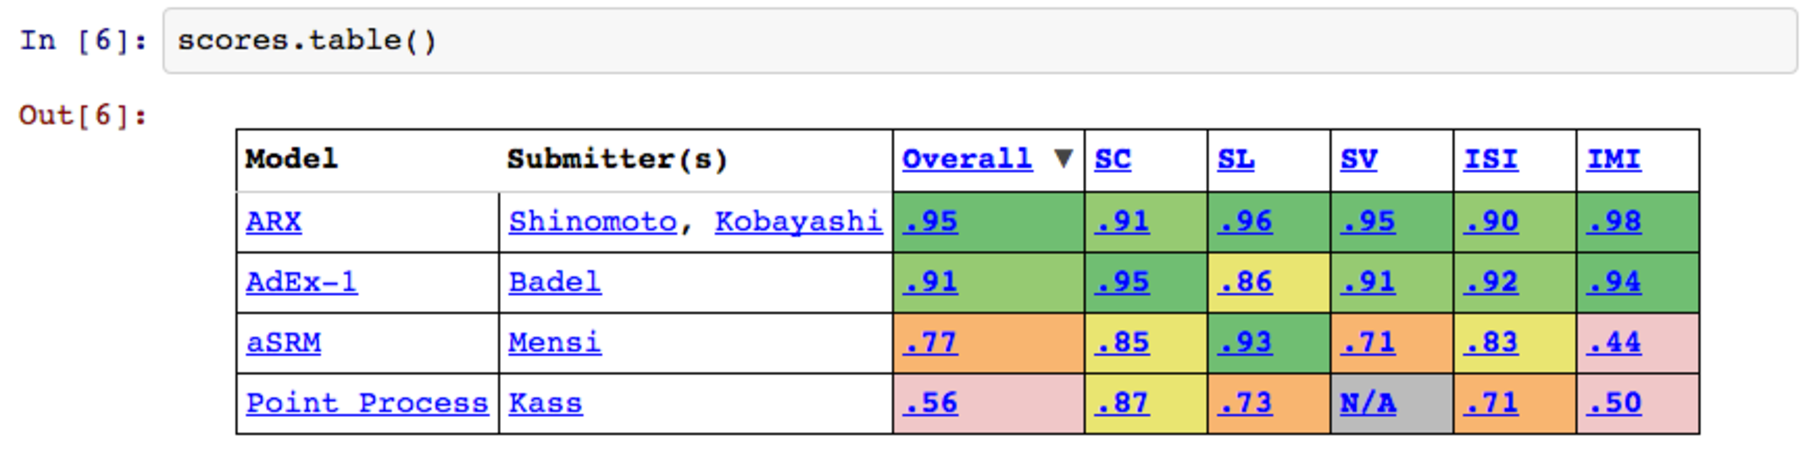
\includegraphics[scale=0.55]{table-ipy.pdf}
\vspace{-10px}
\caption{A score matrix for a SciUnit test suite, visualized as a hyperlinked table inside an IPython notebook stored in a test repository like \textit{hippocampus\_tests}.}
\label{fig:scidash_matrix}
\vspace{5px}
\end{figure}

\section{A Collaborative Workflow}\label{sec:neuronunit_acitivities}
The \textit{NeuronUnit} package contains a collection of test families and associated capabilities relevant to neurophysiology, such as those described in the previous section. 
It is collaboratively developed on Github (\url{http://github.com/scidash/neuronunit}). 
Scientists can use this package to easily create test suites tailored to specific neuronal systems of interest. 
For example, scientists interested specifically in testing models of cells in the hippocampus would use \textit{NeuronUnit} to create tests in a GitHub repository containing an IPython notebook called \textit{hippocampus\_tests}, parameterized by data from the hippocampus.%, parameterizing them by relevant data from \textit{NeuroElectro}. 
%To make this easy, \textit{NeuronUnit} contains \emph{bridge functions} for retrieving data and generating tests from \textit{NeuroElectro} directly (Sec. \ref{sec:neuroelectro}). 

Statisticians interested in improving how goodness-of-fit is measured can simply fork the \textit{NeuronUnit} repository, modify the logic in the relevant test families and submit a \emph{pull request} for evaluation by the community. 
Rather than attempting to convince a large number of scientists socially that the methods used in canonical papers need to be changed, statisticians need only propagate a change to the testing logic used by the community. 
Once the testing logic has been changed, all models can be immediately evaluated against the new metrics. 
Scientists wishing to determine statistical best-practices for measuring goodness-of-fit need only refer to the tests in these repositories.

To submit a new model for testing, a scientist can similarly fork the \textit{hippocampus\_tests} repository, add a new model to the relevant suite and test the model against available tests locally. 
When satisfied with parameter choices, the scientist can submit a pull request to the common repository. 
Once a model is in the repository, it will be evaluated on an ongoing basis against the latest accepted collections of tests, parameterized by the latest data, using the latest statistical best practices, without the participation of the original modeler, assuming only that the capabilities required by the tests stay stable.  

GitHub is an excellent platform for this kind of activity, and is becoming a widely-used tool for scientific collaboration, reproducibility, and transparency \citep{ram_git_2013}.  
We anticipate that other communities within neuroscience (and indeed, within science more broadly) will develop repositories similar to \textit{NeuronUnit} that provide a common, collaboratively-developed vocabulary of test families and capabilities relevant to their domain, and bridge with relevant standardization efforts and infrastructure. 
Using these common repositories, smaller groups of scientists interested in particular systems of interest will develop tests and models in test repositories like \textit{hippocampus\_tests}. 
Each research community can develop suitable quality standards and processes for merging these pull requests. 

The end result of these efforts will be tables, like the one shown in Figure \ref{fig:scidash_matrix}, that allow scientists to understand, precisely, the state-of-the-art in their field. 
We are developing a lightweight portal, \textit{SciDash}, that directs scientists to the canonical test repositories in their field in order to prevent fragmentation and encourage community participation \citep{omar_sciunit_2013}. 
\textit{SciDash} will also facilitate viewing test results without needing to clone test repositories and run tests locally for exploratory purposes, based on the \textit{iPython notebook} technology mentioned in Sec. \ref{sec:visualization}. 
We leave details of \textit{SciDash} as future work, focusing this paper on the core testing methodology (Sec. 2) and on the details of the bridge technologies, below.

\section{Integrating With Neuroinformatics Tools and Infrastructure}\label{sec:neuronunit}
In the examples in the previous sections, tests were provided data explicitly, and models implemented capabilities directly. 
In many fields, however, both models and data are available from existing  community resources in standardized formats. 
In this section, we will show how to use this existing infrastructure to make parameterizing tests with published data and generating \textit{SciUnit} models from models implemented in some other manner (even in a language other than Python) nearly automatic. 
In particular, we will continue to focus on neurophysiology as our initial case study, using machine-readable models written in \textit{NeuroML} available from OpenSourceBrain (\textit{OSB}), and machine-readable data from \textit{NeuroElectro}. 

\subsection{Reference Data for Tests from NeuroElectro}\label{sec:neuroelectro} 
\begin{figure}
\begin{python}
reference_data = neuroelectro.NeuroElectroSummary( # Pooled experimental data from  neuroelectro.org. 
  neuron = {'name':'Hippocampus CA1 pyramidal cell'}, # Neuron type according to NeuroLex ontology.  
  ephysprop = {'name':'Spike Width'}) # Electrophysiological property name in same.
reference_data.get_values()  # Get summary data for the above. 
model = models.OSBModel( # Initialize the model.
        'hippocampus', # Brain area.  
        'CA1_pyramidal_neuron', # Neuron type name in OSB.  
        'CA1PyramidalCell') # Model name (Migliore et al, 2005).
test = SpikeWidthTest( # Initialize the test.    
	reference_data = {'mean':reference_data.mean, 'std':reference_data.std}, # Summary statistics.
	model_args = {'current':40.0*pA}, # Somatic current injection in pA.  
	comparator = ZComparator), # A comparison class that implements a Z-score.  
score = test.judge(model)
\end{python}
\vspace{-15px}
\caption{Working example of testing in \textit{NeuronUnit}. Imports excluded for clarity.}
\label{fig:neuronunit_example}

\end{figure}
The NeuroElectro project (\url{http://neuroelectro.org}) is an effort to make all published data on single cell neurophysiology available in a machine-readable format \citep{tripathy_neuroelectro:_2012}.  
Currently, up to 27 electrophysiological properties are available for 93 cell types, gathered from over 2000 single pieces of published data extracted from tables in published papers. 
We have made it easy to parameterize the test families in \textit{Neuron\-Unit}  using data extracted from the NeuroElectro API. 
Tests can be based upon data from single journal articles, or from ensembles of articles with a common theme (e.g. about a particular neuron type). 
The latter is illustrated in Figure \ref{fig:neuronunit_example}, on lines 1-4. Once data has been retrieved from NeuroElectro, associated statistics (e.g. mean, standard error and sample size) can be extracted to parameterize tests (e.g. a test of spike widths on line 10). Data from NeuroElectro is can be used to validate a variety of basic electrophysiological features of neuron models, including spike width, resting membrane potential, after-hyperpolarization amplitude, etc. \todo{write a sentence or two about its use of the NeuroLex repository}
As NeuroElectro is the only publicly curated source of such data, it represents a key resource facilitating test construction.  

\subsection{Models from NeuroML and OpenSourceBrain}\label{sec:neuroml_models}
NeuroML is a standardized model description language for neuroscience \citep{gleeson_neuroml:_2010}. 
It allows many neurophysiological and neuroanatomical models to be described in a simulator-independent fashion. Some simulators, notably the popular NEURON package (\cite{carnevale_neuron_2006}, \url{http://www.neuron.yale.edu/neuron}), can seamlessly export model specifications as NeuroML. 
Because NeuroML is an XML specification, model descriptions can be verified for correctness and queried for model properties and components. We leverage the latter facilities to expose model capabilities automatically. %NeuroML has proven ideal for model sharing, curation, and for answering both questions about \textit{what a model does} and \textit{how to do it} programatically.  

NeuroConstruct (\cite{gleeson_neuroconstruct:_2007}, \url{http://www.neuroconstruct.org}) is a simulation manager that takes NeuroML models and hands off them off to a supported simulator for execution. A number of popular simulators support execution of NeuroML models, including NEURON, GENESIS (\cite{bower_genesis_2007}, \url{http://genesis-sim.org}), NEST (\cite{gewaltig_nest_2007}, \url{http://www.nest-initiative.org}), and MOOSE (\cite{ray_moose_2008}, \url{http://moose.ncbs.res.in}). 
\textit{NeuronUnit} provides a \verbx{sciunit.Model} subclass called \verbx{NeuroConstructModel} that takes a path to a NeuroML model as a parameter.  
NeuroML can describe a wide range of models, but our \verbx{NeuroConstructModel} class currently supports only  time-integrable point neurons (exposing capabilities \verbx{TimeIntegrable} and \verbx{HasMembranePotential} at minimum; see Sec. \ref{sec:neurotools}). 
It can be instantiated directly or subclassed (useful when additional capabilities need to be manually exposed, for example) to generate a model suitable for testing (Fig. \ref{fig:ca1_model}). The underlying simulator can be configured (defaulting to ??\todo{What does it default to in our code??}; not shown). In this example, we simply create a model based on a NeuroML model of CA1 cells downloaded from OpenSourceBrain to the local file system (\url{http://opensourcebrain.org/projects/ca1pyramidalcell}).  

\textit{OSB} curates many models described in NeuroML. 
OSB-curated projects have been converted from their native format into NeuroML. To ensure that the NeuroML model is faithful to the original simulation, OSB verifies concordance between model output (beginning with the NeuroML description) and reference output (from native simulator source files or published figures) for each model. 
Thus, OSB is an excellent source of models that, in addition to being open source, are known to be accurately described. This also highlights the distinction between \emph{verification} activities, performed by OSB to ensure that a model description operates correctly, and \emph{validation} activites, performed using SciUnit to check the model's predictions against data. Both are important activities.

To directly test a model in OSB, we can skip the step of downloading it the local file system or adding it to the test repository and simply download it from OSB directly by using the \verbx{OSBModel} class, shown on lines 5-8 of Figure \ref{fig:neuronunit_example}. 

%Spanning a range of scales and original development environments, all OSB models are formally described using NeuroML, as are all model components and sub-components, such as cells, ion channels, calcium stores, etc. 
%These models are regularly executed on OSB servers to ensure that their output remains consistent as they are updated. 
%Therefore, OSB can confirm that they \textit{do} work, while linked journal articles, on-site wiki, and code inspection can establish \textit{how} they work. 
%However, there is no mechanism for establishing \textit{how well} they work, i.e. how well the models accord with data. 
%\textit{NeuronUnit} fills this gap by helping OSB (and the larger neuroscience community) assess models using data-driven tests. 
%\textit{SciUnit} can be applied similarly to other neuroscience (or biology) sub-disciplines using \textit{NeuronUnit} analogues written by the corresponding communities.    

\begin{figure}
\begin{python}
class CA1PyramidalCellModel(NeuroConstructModel):
	"""CA1 Pyramidal Cell model in the local file system."""
	def __init__(self):
		project_path = neuroconstruct.get_path("hippocampus","CA1_pyramidal_neuron","CA1PyramidalCell","neuroConstruct")
		NeuroConstructModel.__init__(self,project_path)
\end{python}
\vspace{-15px}
\caption{A model class corresponding to a CA1 Pyramidal Cell model from Open Source Brain}
\label{fig:ca1_model}
\vspace{-10px}
\end{figure}

\subsection{Data Formats and Capabilities from NeuroTools}\label{sec:neurotools}
NeuroTools (\url{http://neuralensemble.org/NeuroTools}) is a Python library supporting tasks associated with analysis of neural data (or model output), such as membrane potential time series, spike trains, etc. 
It is an open source and actively developed project, containing reliable algorithms on which to base neurophysiology tests.

We use NeuroTools to implement a variety of \textit{SciUnit} capabilities in \textit{NeuronUnit}. 
For example, an \verbx{AnalogSignal} object (e.g. a membrane potential time series) from NeuroTools has a threshold detection method that returns a NeuroTools \verbx{SpikeTrain} object. 
The \textit{NeuronUnit} capability \verbx{HasSpikeTrain}  requires that a method named \verbx{get_spike_train} be implemented, returning a \verbx{SpikeTrain} object. 
\verbx{NeuroConstructModel} implements this by default by calling the NeuroTools method \verbx{AnalogSignal.threshold_detection}, retrieving the membrane potential by calling the \verbx{get_membrane_potential} method implemented by the \verbx{HasMembranePotential} capability that all supported NeuroML models implement.
NeuroTools is used in this manner to implement a wide variety of capabilities for \verbx{NeuroConstructModel}s, without requiring that the model developer do so explicitly (though they can overwrite these if they wish). 
This also helps scientists by directing them to a set of common utility functions and data formats that they can use, knowing that they are accepted by the community around NeuronUnit.\todo{do you have a list of capabilities that neuroconstructmodels can automatically implement?}

\section{Discussion}\label{sec:discussion}

\subsection{A Complete Pipeline}
Although the tools described in Sec. \ref{sec:neuronunit} do not exhaust the possible sources of models, capabilities, and test data, they provide an immediate point of entry into the neurophysiology community and a powerful demonstration of our proposal. 
In the \textit{NeuronUnit} repository (\url{http://github.com/scidash/neuronunit}) is a runnable script (\textit{examples.py}) demonstrating a complete testing pipeline. 
It (1) selects an OSB model; 
(2) simulates it using NeuroConstruct; 
(3) tests the widths of the resulting action potentials, extracted and computed using NeuroTools, against NeuroElectro data downloaded on-the-fly, using a \textit{NeuronUnit} test class called \verbx{SpikeWidthTest}; 
and (4) computes and prints a test score (Figure~\ref{fig:neuronunit_example}).


\subsection{Creating New Models, Capabilities, and Tests}
\textit{NeuronUnit} provides base classes to enable rapid generation of models, capabilities, and tests for neurophysiology data. 
However these objects can also be created from scratch, requiring only adherence to the \textit{SciUnit} interface. 
For example, a Model could implement an \verbx{integrate} capability method by wrapping execution of a MATLAB script and a \verbx{get_spikes} capability method by parsing a .csv file on disk; 
a Test could be initialized using empirical spike rates collected in the lab.  
While this does not meet our idealized vision of development and testing, in practice this may be a common scenario. 

\subsection{Participation from Modeling Communities}
Modelers may not want to expose model capabilities, a requirement of test-taking.  
We anticipate four solutions: \textbf{First}, interfacing a model to \textit{SciUnit} requires only implementing selected model capabilities. 
Often this means identifying native model procedures that satisfy a capability, and wrapping their functionality. 
This can require as little as one line of code. 
Importantly, the modeler is not required to expose or rewrite any model flow control. 
\textbf{Second}, we support multiple environments automatically by using NeuroML \citep{gleeson_neuroml:_2010}, and other simulator-independent model descriptions are possible for other domains. 
Automated generation of NeuroML from native model source code is in development (Gleeson, personal communication); for the popular NEURON simulator (\cite{carnevale_neuron_2006}), this functionality is already implemented in use. 
This minimizes modeler effort for a large (at least 1000, \url{http://www.neuron.yale.edu/neuron/node/69}) and growing number of neuronal models. 
\textbf{Third}, modelers have an incentive to demonstrate publicly their models' validity. 
Participation in public modeling competitions demonstrates this incentive. 
\textbf{Fourth}, modelers have an incentive to use \textit{SciUnit} during development (see TDD, above) to ensure that ongoing development preserves correspondence between model and data. 
A popular test suite can represent a ``gold standard'' by which progress during development is judged.

\subsection{Participation from Experimental Communities}
Experimentalists may not want to write tests derived from their data.  
We anticipate four solutions: 
\textbf{First}, tests require no special data formatting; only a list of required  capabilities (for selecting eligible models), optional metadata (as run-time arguments), and a statistical data summary (for scoring tests) are required. 
A unit test is focused and does not require arbitrary computations on data. 
For example, suppose intracellular current injection evokes 100 action potentials, the width of which is of interest. 
Writing the test consists of selecting \verbx{ReceivesCurrent} and \verbx{ProducesActionPotentialShape} capabilities (one line of code each), computing the mean and variance of action potential widths (one line of code), specifying current injection parameters, e.g. amplitude and duration (two lines of code), and selecting a scoring mechanism from \verbx{sciunit.scores}, e.g. (colloquially) ``Must be $<$ 1 standard deviation of the mean'' (one line of code). 
This example can be found in \verbx{NeuronUnit.tests.SpikeWidthTest}; heavy-lifting is done by the interface.
\textbf{Second}, data-sharing is becoming accepted, and test-writing can be distributed across scientists, including non-experimentalists with other aims such as analysis or modeling. 
\textbf{Third}, many tests can be automatically generated using NeuronUnit, and the continued emergence of data-aggregation initiatives such as NeuroElectro will expand these possibilities. 
\textbf{Fourth}, an incentive to write tests for one's data exists: the ability to identify models that give the data clear context and impact. 

\subsection{Diversity of Levels and Kinds of Models and Data}
The diversity of topics in biology is vast. 
\textbf{First}, we address this by providing an interface allowing modelers to express specific capabilities.  
This capability set determines the range of eligible tests.  Scale hierarchies are embedded in capability inheritance. 
For example, \verbx{HasActionPotentials} inherits from \verbx{HasNeurons}, and \verbx{HodgkinHuxley} inherits from \verbx{VoltageGated}. 
Thus, incompatibility of a test-requiring-action-potentials for a model-lacking-neurons is known without explicit tagging. 
\textbf{Second}, NeuroML naturally addresses diversity of scales because it is organized hierarchically, in ``levels.''  
Models can be sub- or supersets of other models; similarly for SBML (\cite{hucka_systems_2003}, \url{http://sbml.org}) a general systems biology markup language. 
\textbf{Third}, cross-level testing can use ``Representional Similarity Analysis'' (RSA) \citep{kriegeskorte_representational_2008}, requiring only that a model respond to defined inputs (e.g. stimuli). 
A ``similarity matrix'' for input responses defines a unique model signature, and can serve as intermediate test output. 
Goodness-of-fit between similarity matrices for model and experiment determines test scores; 
these matrices are independent of model scale because their size depends only on test inputs, not system detail.  

\subsection{Arbitrary Scoring Criteria for Tests}
A test first assesses goodness-of-fit, and applies a normalization (e.g. pass/fail, 0.0-1.0) to generate a score. 
Arbitrary choices at both stages may benefit some models over others. 
\textbf{First}, however, rank-ordering is constant across many goodness-of-fit metrics, meaning that choice of metric will rarely cause an otherwise passing model to fail and vice versa. 
For example, given a data mean and variance, ordering model output by Z-score or p-value will yield the same relative ranking of models. 
Indeed, rank ordering of models may prove more valuable than test scores themselves. 
\textbf{Second}, suite repositories should be open, so tests can be cloned and new statistical choices implemented. 
Statistics as applied to neuroscience have been notoriously ``fast and loose''; 
identification and correction of flawed methodology is becoming increasingly common (\cite{button_power_2013,kriegeskorte_circular_2009,galbraith_study_2010}, \url{http://prefrontal.org/files/posters/Bennett-Salmon-2009.jpg}), and is accelerated by an open framework. 
The validation criteria is made explicit in the specification of a test, so modelers need not guess which criteria are being used to validate or invalidate their model. 
Validation criteria are subject to debate (indeed, the QSNMC criteria changed between 2007 and 2008 due to such debates), and neuroscientists who wish to promote different criteria need only derive alternative tests. 
A community consensus will slowly emerge in the form of commonly-accepted test suites. 
Such a community can judge which test version is most appropriate, i.e. what a model \textit{should} do -- this process documented via standard moderation techiniques used e.g. on GitHub. 
This process can be made even more visible by storing the output of test runs using Sage or IPython worksheets, or through optional database backends such as in the Sumatra lab notebook for simulation and analysis (\cite{sumatra_davison_2012}, \url{http://neuralensemble.org/sumatra}).

\subsection{Reliability of Data Underlying Tests}
Unreliable data can undermine model validation. 
\textbf{First}, the community must evaluate experimental design and methods, discounting data produced using questionable techniques. 
Open source version control services such as GitHub support community moderation, permitting users to comment on tests, indicating their concerns. 
Suite repository popularity can reflect consensus. 
Experimental metadata also constrain a test's relevance, so test writers should select data with metadata appropriate to the system being modeled, and attach the metadata to resulting test scores. 
Using the NeuroElectro API, for example, it is possible to select only data corresponding to specific experimental conditions, for example recording electrode type.  
Metadata can also be expressed as Capabilities, e.g. \verbx{At37Degrees} or \verbx{Calcium3mM}; and tests can require that models express them. 
Such capabilities require no implementation, so the model definition must only inherit them. 
\textbf{Second}, models cannot perfectly reproduce data that is itself a random draw from a ``true'' distribution. 
Uncertainty in data must be made explicit, by asking how well a data set validates its own experimental replications \citep{kriegeskorte_representational_2008}. 
The degree of such ``self-validation'' represents the upper limit of what a model can be expected to achieve, and should represent a ``perfect'' score.  

\subsection{Occam's Razor}
All things being equal, simpler models are better. 
Model complexity has many definitions \citep{mccabe_complexity_1976}, including: 
1) model length; 2) memory use; 3) CPU load; 4) \# of capabilities. 
Future \textit{SciUnit} tools will report the model validity vs complexity tradeoff in tabular form (e.g. Figure \ref{fig:scidash_matrix}), and in a scatter plot, with the ``best'' models being in the high validity / low complexity corner of the plot. 
The set of models which \textit{dominate} all others, i.e. that have the highest validity for a given complexity, can be represented as a ``frontier'' in such a scatter plot, a visualization familiar from the symbolic regression package Eureqa \citep{schmidt_distilling_2009}.  

\subsection{Expansion Into Other Areas of Biology}
After covering neurophysiology with continued development of \textit{NeuronUnit}, we would like \textit{SciUnit} to be applied across neuroscience and in other biological sciences. 
The framework is discipline-agnostic, so community participation and model description are the only obstacles. 
Community participation begins with enumerating the capabilities relevant to a sub-discipline, and then writing tests. 
Model description can expand within NeuroML (which already covers multiple levels within neuroscience) and tools for capability implementation can incorporate libraries for neuroimaging (NiBabel, \url{http://nipy.org/nibabel}), neuroanatomy (NeuroHDF, \url{http://neurohdf.readthedocs.org}) and other sub-disciplines. 
SBML will enable expansion beyond neuroscience, facilitated by parallel efforts among NeuroML developers to interface with it (Crook, unpublished). 
One intriguing possiblity is applying \textit{SciUnit} to the OpenWorm project (\url{http://www.openworm.org}), which through open, collaborative development seeks to model the entire organism C. elegans.  

\section*{Disclosure/Conflict-of-Interest Statement}
%All relationships financial, commercial or otherwise that might be perceived by the academic community as representing a potential conflict of interest must be described. If no such relationship exists, authors will be asked to declare that the research was conducted in the absence of any commercial or financial relationships that could be construed as a potential conflict of interest.
The authors declare that the research was conducted in the absence of any commercial or financial relationships that could be construed as a potential conflict of interest.

\section*{Acknowledgements}
We thank Sharon Crook, Jonathan Aldrich, Shreejoy Tripathy, and Padraig Gleeson for their support of this project.  
The work was supported in part by grant R01MH081905 from the National Institute of Mental Health. 
The content is solely the responsibility of the authors and does not necessarily represent the official views of the National Institutes of Health.

%\bibliographystyle{frontiersinSCNS&ENG} % for Science and Engineering articles
\bibliographystyle{frontiersinSCNS&ENG} % for Medicine articles
\bibliography{references,references_crook,urls,references_ja}

%\bibliographystyle{unsrt}
%\bibliography{references,references_crook,urls,references_ja}
%\listoftodos
\end{document}

